c\section{Validation}

In this section we describe the validation process of the claims made in this proposal.

\begin{enumerate}
\item The first claim made in this proposal is that a computation graph is a suitable representation of the execution of task parallel programs. This proposal uses Habanero Java language to describe the implementation details. Using the semantic model for parallel programming languages described in \cite{bouajjani2012analysis}, we can be show that Habanero Java is a superset of other task parallel languages. It contains a wide range of parallel programming constructs that can be used to perform all operations that are possible in other task parallel languages such that Cilk, Chapel, OpenMP3.0, X10 etc. Now, in this section, we describe how to create computation graphs for other task parallel languages. The analysis of these computation graphs proceeds in the same way as analysis of computation graphs for Habanero Java programs. The following examples illustrate the computation graphs for programs written in different task parallel languages.

\begin{enumerate}
\item 
\textbf{X10}
\begin{figure}[H]
\centering
\begin{minipage}[b]{0.35\linewidth}
    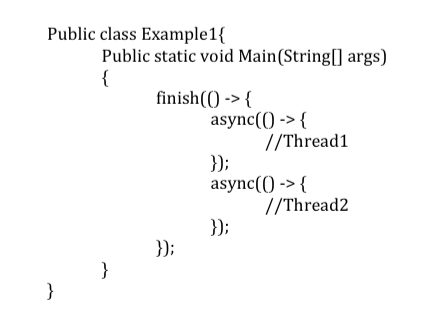
\includegraphics[scale=0.4]{../figs/X10.jpg} 
\caption{X10 Program}
\label{fig:minipage3}
\end{minipage}
\quad
\begin{minipage}[b]{0.35\linewidth}
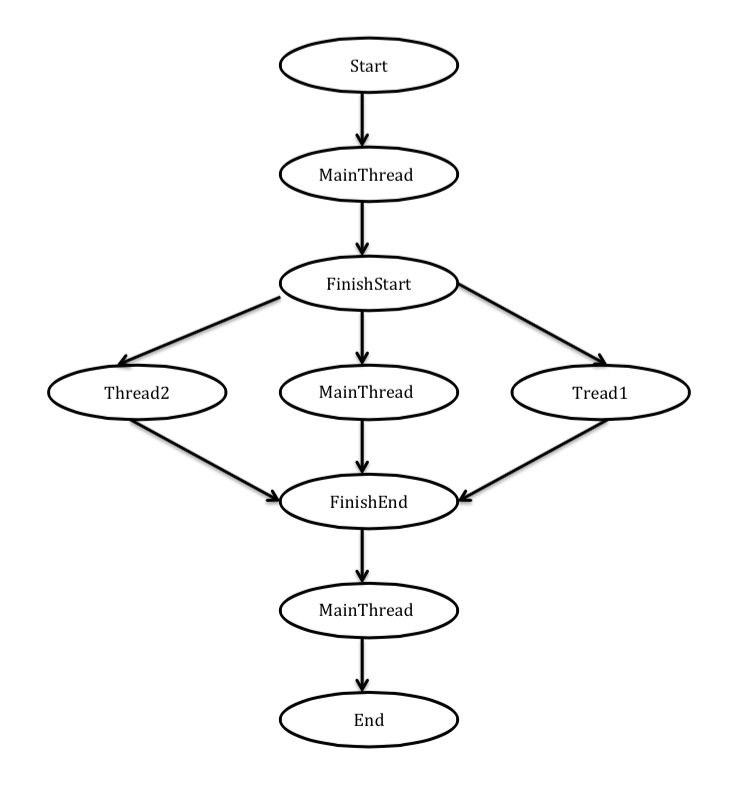
\includegraphics[scale=0.2]{../figs/X10_CG.jpg}
\caption{CG of X10 Program}
\label{fig:minipage4}
\end{minipage}
\end{figure}

\item
\textbf{OpenMP3.0}
\begin{figure}[H]
\centering
\begin{minipage}[b]{0.35\linewidth}
    \includegraphics[scale=0.2]{../figs/Openmp.jpg} 
\caption{Openmp Program}
\label{fig:minipage5}
\end{minipage}
\quad
\begin{minipage}[b]{0.35\linewidth}
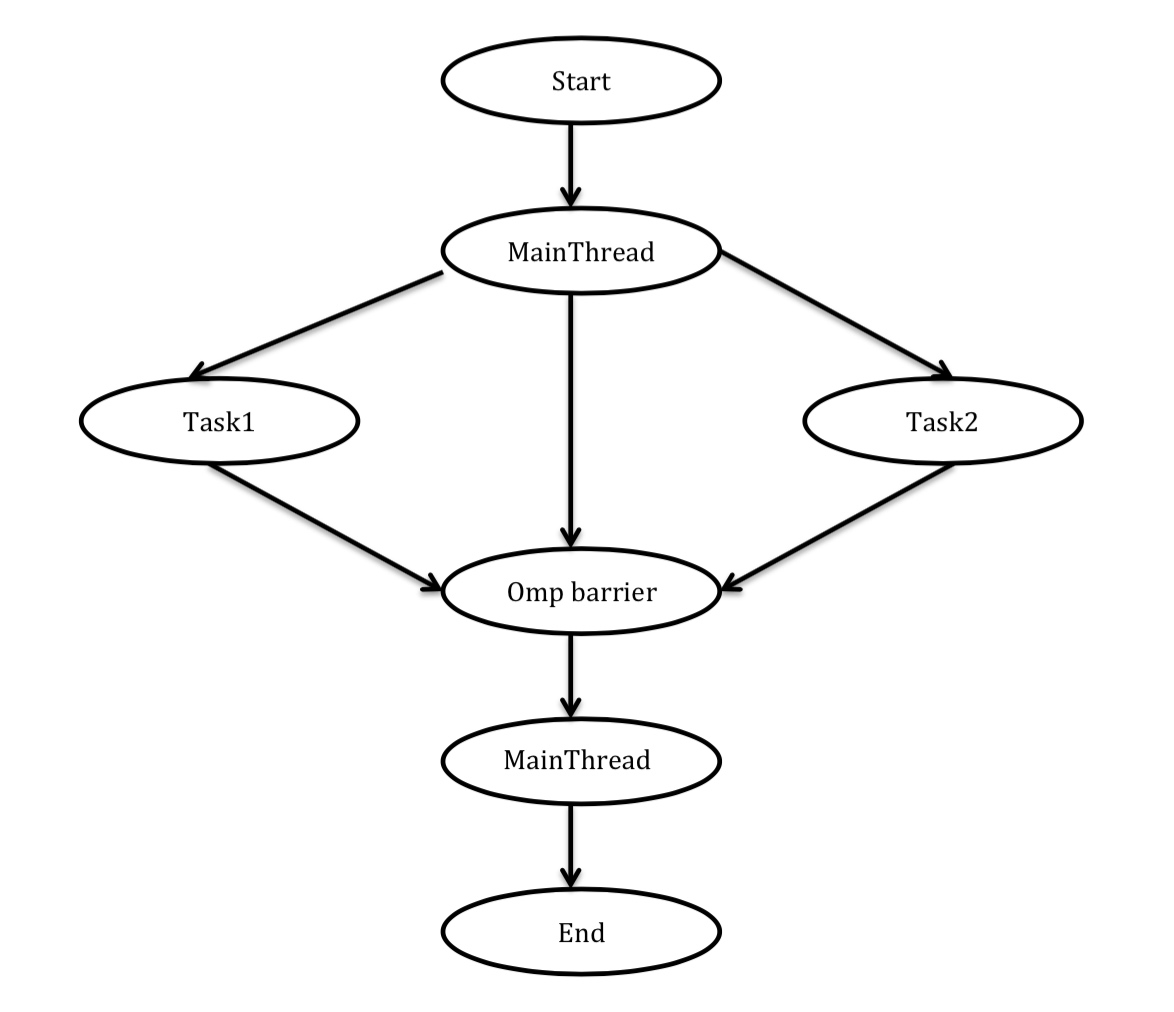
\includegraphics[scale=0.1]{../figs/openmp_CG.jpg}
\caption{CG of Openmp Program}
\label{fig:minipage6}
\end{minipage}
\end{figure}

\item
\textbf{Cilk}
\begin{figure}[H]
\centering
\begin{minipage}[b]{0.35\linewidth}
    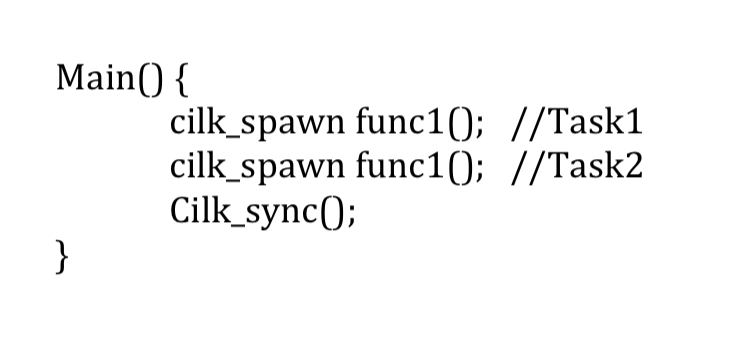
\includegraphics[scale=0.2]{../figs/Cilk.jpg} 
\caption{Cilk Program}
\label{fig:minipage7}
\end{minipage}
\quad
\begin{minipage}[b]{0.35\linewidth}
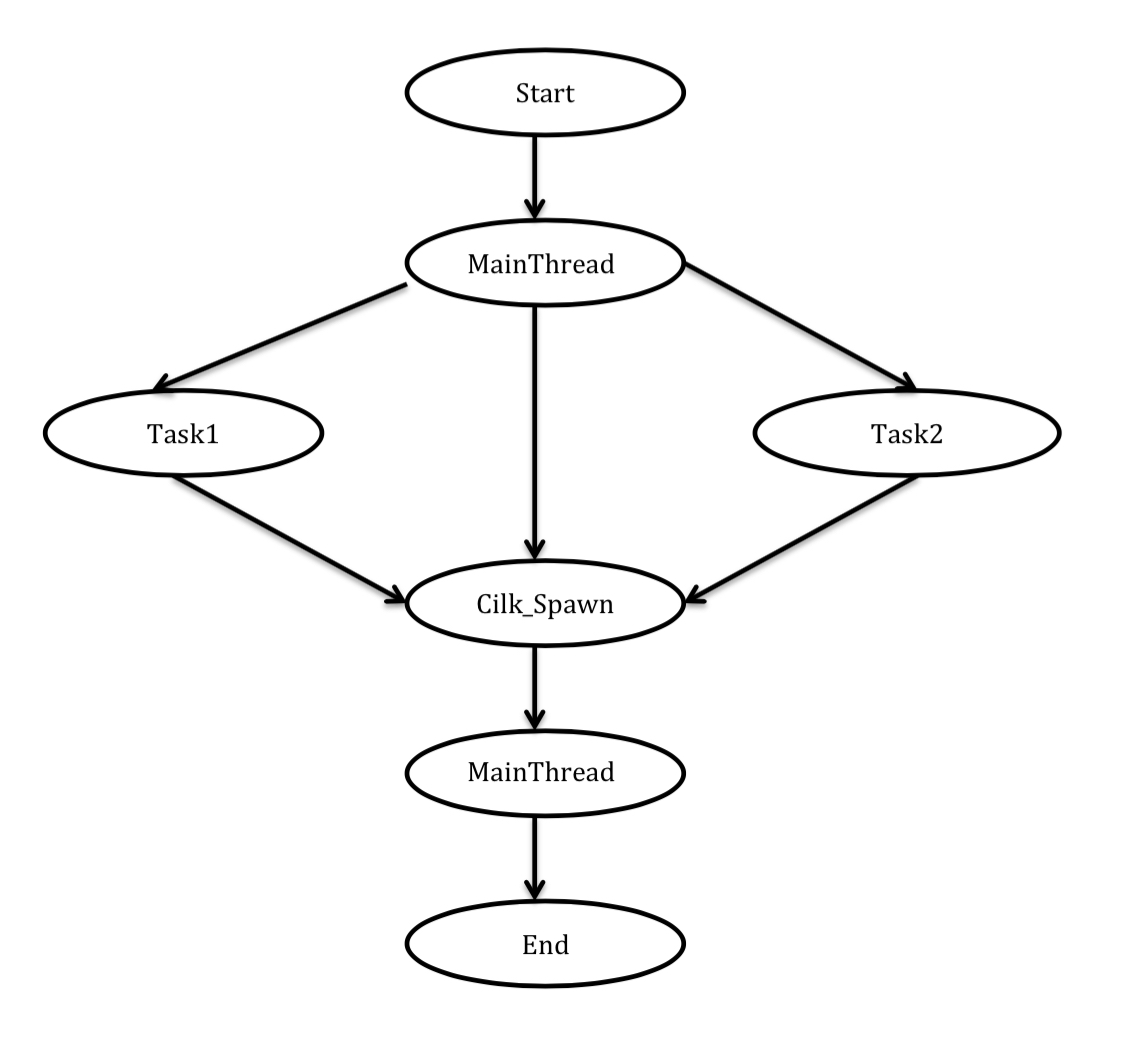
\includegraphics[scale=0.1]{../figs/Cilk_CG.jpg}
\caption{CG of Cilk Program}
\label{fig:minipage8}
\end{minipage}
\end{figure}

\item
\textbf{Chapel}
\begin{figure}[H]
\centering
\begin{minipage}[b]{0.35\linewidth}
    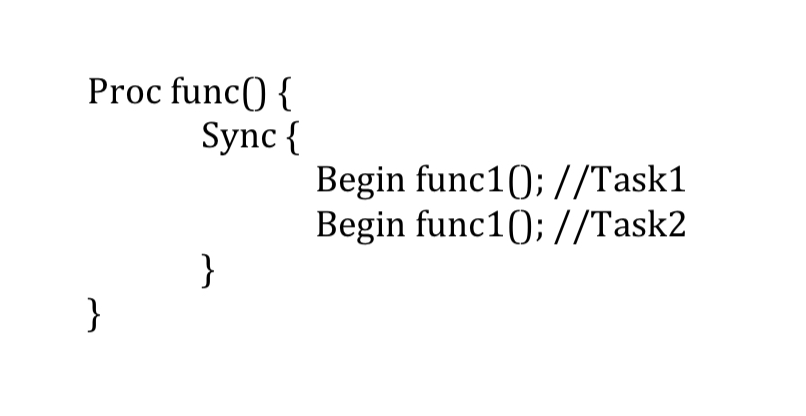
\includegraphics[scale=0.2]{../figs/Chapel.jpg} 
\caption{Chapel Program}
\label{fig:minipage9}
\end{minipage}
\quad
\begin{minipage}[b]{0.35\linewidth}
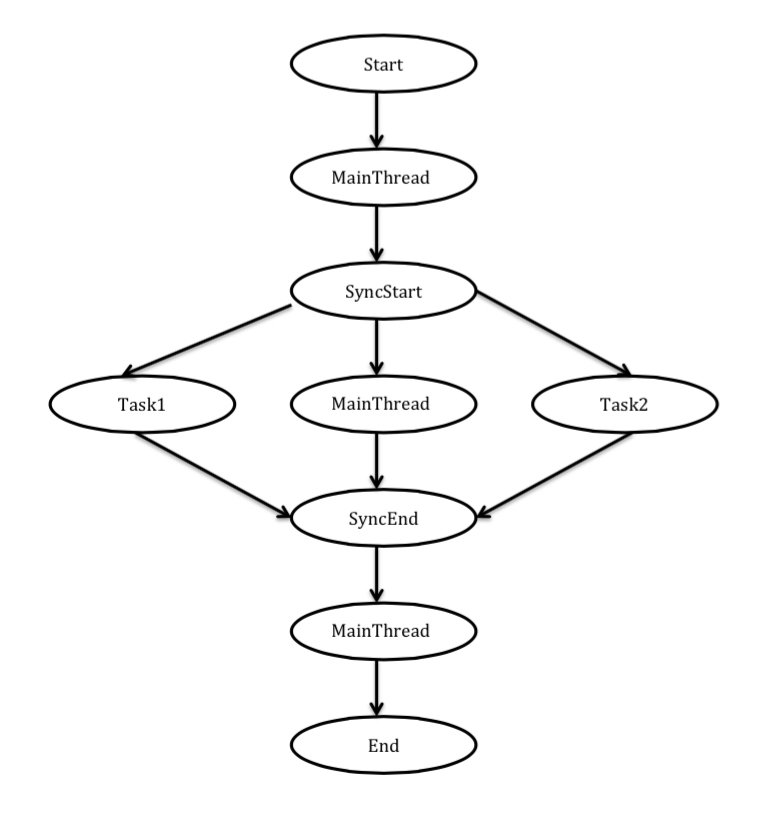
\includegraphics[scale=0.1]{../figs/Chapel_CG.jpg}
\caption{CG of Chapel Program}
\label{fig:minipage10}
\end{minipage}
\end{figure}
\end{enumerate}

\item The second claim is that a computation graph can determine all relevant schedules over tasks that are necessary to be validated to enumerate the possible behaviors of the program. From the implementation details of the computation graph creation, we can see that in the absence of co-ordination constructs such as 'isolated' that do not impose ordering over the concurrent events or tasks, only one schedule needs to be checked to verify the behavior of the program. In programs involving co-ordination over tasks, the computation graph marks the events that have to be ordered and inserts serialization edges between them. The analysis of the program takes into account the specific ordering of the events and creates schedules such that each of the event ordering is considered in such programs.

To test the correctness of this approach, we have selected benchmarks from the Java Grande Forum benchmarks (JGF) suite, Barcelona OpenMP Task Suites benchmarks (BOTS), Shootout benchmarks suite, and EC2 challenge. These benchmarks include programs that exhibit both kinds of behaviors(single computation graph for programs without co-ordination constructs and multiple computation graphs for programs with co-ordination constructs). The Nqueens and Matrix multiplication benchmarks demonstrate the use of basic parallel programming constructs such as async-finish and loop parallelism constructs such as foreach and forall. The Frannkuch and Mandelbrot benchmarks makes use of the co-ordination construct Isolated in conjunction with the simpler async-finish parallel constructs. The LUFact, SOR and MolDyn benchmarks focus on the co-ordination constructs such as phasers and futures. The BOTS  benchmarks from the Barcelona OpenMP Task Suites focus on various parallel constructs of OpenMP. They have been suitably ported to Habanero Java  to be verified with this tool. The following table lists out the benchmarks that are going to be used for validation. 

\begin{tabular}{|c|c|c|}
\hline
\textbf{Source} & \textbf{Benchmark} & \textbf{Description} \\
\hline
\hline
      & Crypt & IDEA encryption \\
	& LUFact C & LU Factorization \\
  	   & MolDyn & Molecular Dynamics simulation \\
JGF & MonteCarlo & Monte Carlo simulation \\
      & RayTracer & 3D Ray Tracer \\
      & Series & Fourier coefficient analysis \\
      & SOR & Successive over-relaxation \\
      & SparseMatMult & Sparse Matrix multiplication \\
      \hline
      & FFT  & Fast Fourier Transformation \\
	Bots & Health & Simulates a country health system \\
& Nqueens & N Queens problem \\
& Strassen & Matrix Multiply with Strassen’s method \\
\hline
Shootout & Fannkuch & Indexed-access to tiny integer-sequence \\
& Mandelbrot & Generate Mandelbrot set portable bitmap \\
\hline
EC2 & Matmul & Matrix Multiplication \\
\hline
\end{tabular}

\item The third claim made in this proposal is that an exhaustive enumeration of all possible behaviors of a program made with the help of computation graphs is enough for verifying deterministic behavior in task parallel programs. To validate this claim, we use the micro-benchmarks in Habanero Java described in the table below. These micro-benchmarks represent each of the different possible behaviors that can be observed in task parallel programs. A program that is data-race free is always structurally and functionally deterministic. The first example belongs to this category. The second example contains data-races but the program is structurally and functionally deterministic. The third example also has a data-race. The program is structurally deterministic since the program spawns the same number of tasks in every run but functionally non-deterministic because the index of the search term will be different when the searched text has multiple occurrences of the query. The fourth example has data races and is functionally deterministic. But, the program is structurally non-deterministic since number of new spawned tasks depend on the occurrence of the query. The last example has data-races and exhibits both structural and functional non-determinism. This list of micro-benchmarks includes all possible behaviors that a task parallel program can exhibit. The third claim can be validated if the implementation described in this proposal can correctly determine the category for these programs. 

\begin{tabular}{ | c | c | c | c |}
  \hline
  \textbf{Test Case} & \textbf{Data Race Free} & \textbf{Structurally deterministic} & \textbf{Functionally deterministic} \\
  \hline
  Search Count & Y & Y & Y \\
  \hline
  Search & N & Y & Y \\
  \hline
  Search Index & N & Y & N\\
  \hline 
  Search Index With No TaskCreation & N & N & N\\
   after Instance is Found  & & & \\
  \hline 
\end{tabular}
\\
\\
We are going to measure the number of the states explored by this implementation and compare it to the number of states explored by JPF's data-race detector. It is expected that this implementation will explore less number of states to detect data-races. We are also going to compare the runtimes of this method to JPF's data race detector to measure performance improvement.

\end{enumerate}